\chapter{Results}\label{results}
	This chapter discusses the performance of the two developed algorithms in sections \ref{result_profiles} and \ref{result_curves}. In section \ref{bubble_distributions}, bubble distributions computed with algorithms \ref{algo:bubbleNet} and \ref{algo:bubbleCurves} are discussed. 
	
		\section{BubbleProfiles}\label{result_profiles}
			
			After training for 14 epochs, the testing accuracy converged to 96.8\%, which is a very good result for a binary classifier. 

			For validation, 20 more manually annotated small images were used, each containing from 10 to 20 bubbles. Figure \ref{fig:bubbleNet_result} illustrates the performance of algorithm \ref{algo:bubbleNet}.  
			The algorithm achieved mAP@.5IoU = 91.5\% and mAP@.3IoU = 93\%. Note that this is slightly worse than the classification accuracy result. This is due to the occasionally unprecise radius computation, which gets penalized by the mAP@p-IoU criterion. 
			
			\begin{figure}[h!]
				\centering
				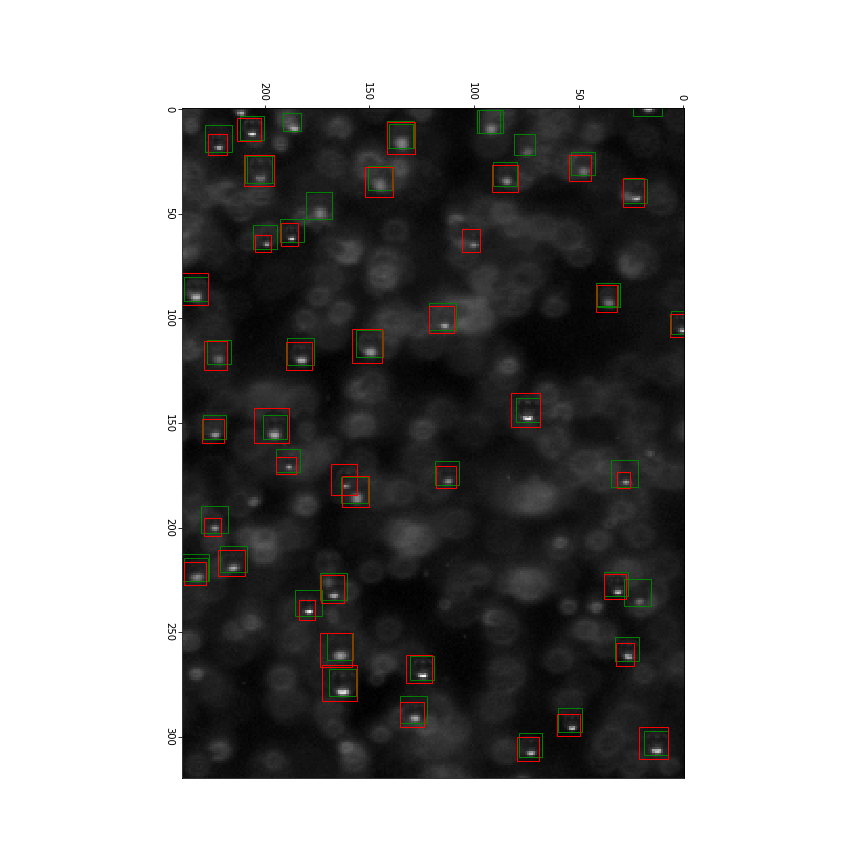
\includegraphics[scale=0.8]{images/bubbleNet_validation_result.png}
				\caption{Testing of algorithm \ref{algo:bubbleNet}. Red: ground truth, green: predicted. Note how in this image, ground truth annotation was not done perfectly, so IoU results were likely slightly underestimated.}
				\label{fig:bubbleNet_result}
			\end{figure}





			\section{BubbleCurves}\label{result_curves}
				\begin{figure}[h!]
					\centering
					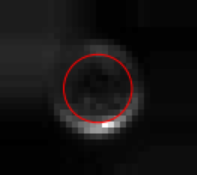
\includegraphics[scale=1.3]{images/bubbleCurve_final_result.png}
					\caption{Final result of algorithm \ref{algo:bubbleCurves} applied to a single bubble}
					\label{fig:final_result}
				\end{figure}
				
				The final result is shown in figure \ref{fig:final_result}. Although the circle matches the bubble's shape well, it is clear that the radius has been underestimated. Similarly to algorithm \ref{algo:bubbleNet}, radius calibration is addressed in section \ref{sub:radius_algorithm}
				
				Using a validation set of 30 small images, each containing 30 to 40 bubbles, this algorithm achieved mAP@.5IoU = 89.3\%, which is slightly worse than algorithm \ref{algo:bubbleNet}. This is in part due to the high rate of overlap between bubbles, making curvature extraction less precise.. Nevertheless, the algorithm is reliable enough to be usable for bubble detection in high concentration images.					
				
				\section{Bubble distributions}\label{bubble_distributions}